\newpage
\section{Digital signal processing}
\subsection{Digital representation of a continuous signal}
Assume a signal $y(t)$ (e.g., a voltage) which varies continuously in time. To store and process this signal on a computer we measure it at a set of time instants $t_i$ yielding values of the signal $y_i$, resulting in the discrete representation of the signal as a series of pairs $(t_i, y_i)$. The signal is uniformly sampled if $t_i = i\Delta t$, where $\Delta t$ is the \textbf{sampling period} and $f_s = 1/\Delta t$ is the \textbf{sampling frequency}.

Any information about the original signal $y(t)$ that varies in time faster than $\Delta t$ is lost. However, if $y(t)$ oscillates at a frequency $f$ it is insufficient to have $f_s \geq f$. Signal frequencies $f > f_s/2$ will appear shifted to $f - f_s/2$, see the output of Lst.~\ref{ls:label}. The sampled signal contains fictitious frequencies which are not present in the original signal. 

This distortion is called \textbf{aliasing} and the \emph{Nyquist theorem} states that in order to avoid aliasing, the highest frequency contained in the signal $f$ must not be higher than one half of the sampling frequency $f_s/2$, which is called the \textbf{Nyquist frequency} 
\begin{equation}
    \label{eq:nqyust}
    f_N = f_s/2.
\end{equation}

\lstinputlisting[caption=Effect of sampling rate, label=ls:label]{../example_code/sampling.py}
\begin{center}
    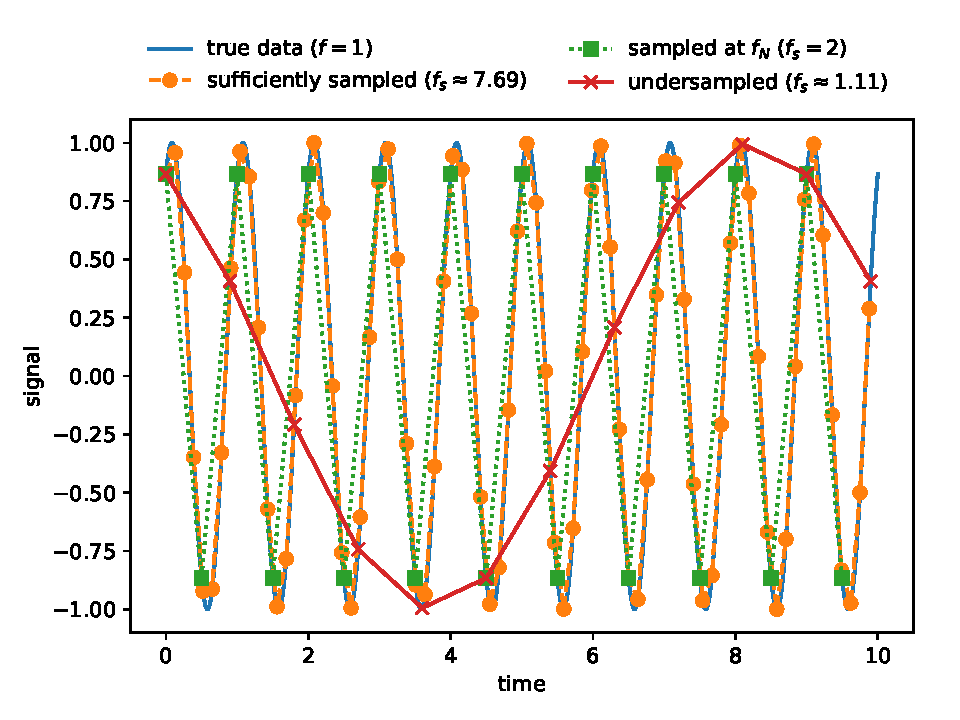
\includegraphics[width=0.75\linewidth]{sampling.pdf}
\end{center}

\subsection{Spectral analysis}
Any periodic signal $y(t)$ (which can be complex) with a period $T$, i.e., $y(t + T) = y(t)$, can be represented as a sum of sine and cosine terms oscillating at angular frequencies $2\pi n/T$ where $n$ is an integer,
\begin{equation}
    y(t) = \frac{1}{T} \sum_{k=0}^{\infty} A'_k\sin\left(\frac{2\pi k}{T}t\right) + B'_k\cos\left(\frac{2\pi k}{T}t\right),
\end{equation}
which is called the \textbf{Fourier series}. Equivalently, the Fourier series can be expressed using complex exponentials
\begin{equation}
    y(t) = \frac{1}{T} \sum_{k=-\infty}^\infty A_k e^{2\pi ikt/T},
\end{equation}
where for a real signal $y$ the positive and negative terms are complex conjugate, $A_k = A_{-k}^*$ (the $1/T$ factor and sign inside the exponential function are conventional).

Fourier coefficients $A_k$ can be calculated as
\begin{equation}
    A_k = \int_0^T y(t) e^{-2\pi ikt/T} \mathrm{d}t
\end{equation}

For example, consider the directly-calculated Fourier series in Lst.~\ref{lst:fourier-square-pulse}
\lstinputlisting[label=lst:fourier-square-pulse, caption=Fourier series of a square pulse.]{../example_code/fourier_series_square_wave.py}
\begin{center}
    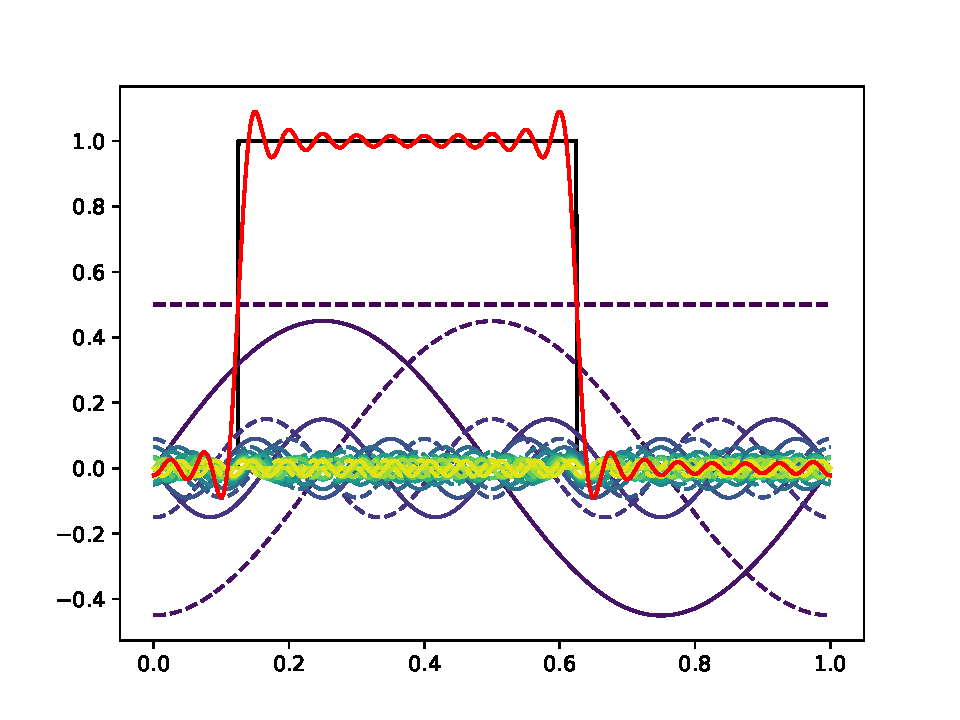
\includegraphics[width=0.5\linewidth]{fourier_series_square_pulse.pdf}
\end{center}

These definitions can be extended to aperiodic signals (which can be imagined as signals with infinitely long periods) which yields the \textbf{Fouerier transform}
\begin{equation}
    \tilde y(\omega) = \int_{-\infty}^\infty y(t)e^{-i\omega t} \mathrm{d}t,
\end{equation}
and the \textbf{inverse Fourier transform}
\begin{equation}
    y(t) = \frac{1}{2\pi}\int_{-\infty}^\infty \tilde y (\omega)e^{i\omega t}\mathrm{d}\omega
\end{equation}

The absolute value of the Fourier coefficients $|A|$ is the amplitude of the signal's oscillation at a given frequency and their complex phase is the phase rotation of the sine and cosine terms. For the Fourier transform, since the frequency now varies continuously, the $|\tilde y|$ has a meaning of \emph{density} (called spectral density). In analogy with electrical power $P = V^2/R$ needed to generate voltage $V$ across a resistor $R$, $|\tilde y|^2$ is called the \emph{power spectral density}, i.e., $\int_{\omega_0}^{\omega_1} |\tilde y (\omega)|^2\mathrm{d}\omega$ is the power of the signal in the frequency band $(\omega_0, \omega_1)$.

For digital signals, we talk about \emph{discrete} Fourier transforms. For uniformly sampled signals, $t_n = n\Delta t$ these are in SciPy defined as (in the submodule \ls{scipy.fft})
\begin{equation}
    \tilde y[k] = \sum_{n=0}^{N-1}y[n]e^{-2\pi i kn/N},
\end{equation}
where $y[n]$ is the value of the signal $y$ measured at time $t_n = n\Delta t$ and $N$ is the total number of samples. The dimensionless integer frequencies $k$ run from 0 to $N-1$ -- that is, the fourier transform has the same length as the original signal. 

The inverse discrete Fourier transform is defined similarly,
\begin{equation}
    y[n] = \frac{1}{N}\sum_{k=0}^{N-1}\tilde y[k]e^{+2\pi i kn/N}.
\end{equation}

The integer frequency indices $k$ represent frequencies $f'_k = k/N$ for $k=0\dots N/2$ and $f'_k = -k/N$ for $k=N/2\dots N-1$. To get the actual frequencies we only need to scale $f'_k$ with the actual sampling frequency $1/\Delta t$. Notice that the definitions of the discrete Fourier transform and its inverse do not depend on the sampling rate, only on the fact that the signal is sampled uniformly.

Fourier transforms are implemented in NumPy and SciPy using the \textbf{Fast Fourier Transform -- FFT} algorithm\footnote{FFT is one of the most important algorithms that the entire digital world depends on -- e.g., sound and video encoding and wireless communication rely on it heavily.} in the \ls{scipy.fft} submodule. Fourier transform is calculated using \ls{scipy.fft.fft()} and the actual frequencies can be calculated using a helper function \ls{scipy.fft.fftfreq()}. Both \ls{fft} and \ls{fftfreq} return positive and negative frequencies. For real signals, the negative frequencies do not provide any extra information therefore we can use \ls{scipy.fft.rfft()} and \ls{rfftfreq()} which return only positive frequencies (i.e., the result is half the length of the original signal). If we are only interested in the power spectral density, there is \ls{scipy.signal.periodogram()} which also calculates the frequencies. By default, for real signals, \ls{periodogram} returns only the positive frequencies and both positive and negative frequencies for complex signals. See Lst.~\ref{lst:fouriers} for example usage and Lst.~\ref{lst:fft-square-wave} for a version of the program in Lst.~\ref{lst:fourier-square-pulse} but using FFT rather than manual calculation of the coefficients

\lstinputlisting[caption=Calculation of Fourier transform and power spectral density., label=lst:fouriers]{../example_code/fouriers.py}
\begin{center}
    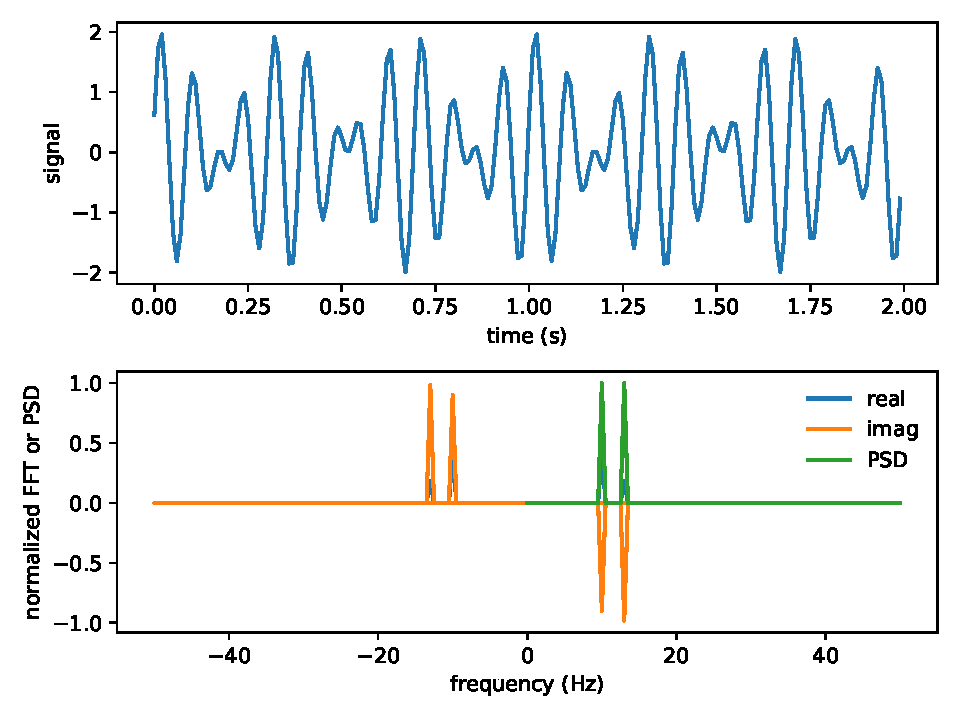
\includegraphics[width=0.5\linewidth]{fouriers.pdf}
\end{center}

\lstinputlisting[label=lst:fft-square-wave, caption=Fourier coefficient of a square wave\, calculated using FFT]{../example_code/fourier_series_square_wave_fft.py}

One particularly important Fourier transform is that of the exponentially decaying oscillation, i.e.
\begin{equation}
    s(t) = e^{-t/\tau}\sin(2\pi f t),
\end{equation}
which yields the complex lorentzian which is the response of the linear harmonic oscillator, see Sec.~\ref{sec:lho}. The decaying oscillation is, of course, the motion of the damped unforced linear harmonic oscillator. Example:
\lstinputlisting[caption={Fourier transform of a decaying sine wave.}]{../example_code/decaying_exponential.py}
\begin{center}
    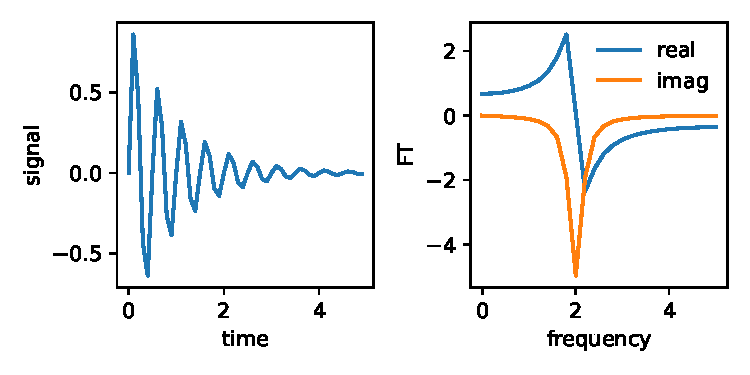
\includegraphics{decaying_exponential.pdf}
\end{center}

\begin{syntax}[Storing data and metadata in numpy binary files.]
    \label{syn:npy}
    So far, when loading data from a disk, we encountered only simple human-readable text files. This is a very limiting way to store data: the data have to have the form of a rectangular table, the files take up more space than necessary (e.g., text \ls{1.234567890} requires 11 bytes of memory but a \ls{float} representing the same number only needs 8), and it is cumbersome to store metadata.

    Many file formats address these issues (e.g., HDF5 is popular). Here we will use a solution that does not require any further external libraries -- storing dictionaries in compressed binary \ls{.npy} files, e.g. saving
\begin{lstlisting}
    raw_data = np.linspace(0, 1, 50)
    my_data = {
        'date of measurement': '20241224',
        'was Mercury in retrograde': False,
        'data': raw_data
    }
    np.save("my_data.npy", my_data)
\end{lstlisting}
    and loading
\begin{lstlisting}
    my_data = np.load("my_data.npy", allow_pickle=True).item()
    print(my_data['date of measurement'])
    print(my_data['data'])
\end{lstlisting}

    \textbf{Pickling} is a Python term for storing almost any Python object on disk as binary data. Loading a pickled object can in, some circumstances, be a security risk (i.e., avoid reading pickled data you downloaded from weird places on the internet), therefore we have to allow it explicitly. Functions \ls{np.load} and \ls{np.save} are working with arrays, therefore \ls{np.load()} returns an array of length 1 where our dictionary is the only element. The method \ls{array.item()} returns \ls{array[0]} if \ls{array} is length 1 or raises a \ls{ValueError} exception otherwise. Its purpose is to semantically indicate that we expect the array to only have one element and if it does not, something is wrong.
    
    \begin{exercise}
    Read data from the directory \ls{timeseries_data} and plot the time-dependence of the approximate mean temperature during the measurement. Read the files using \ls{d = np.load(filename, allow_pickle=True).item()}. The temperature at the beginning and end of the measurement period is \ls{d['Ti']} and \ls{d['Tf']}, respectively.
    
    \emph{Hint:} To get the timestamp (number of seconds since 00:00 1.1.1970) you can use \ls{time.mktime(time.strptime(fn, 'DM_\%Y\%m\%d-\%H\%M\%S.npy'))}, with \ls{fn} the filename.
\end{exercise}
\end{syntax}

\begin{exercise}
    Plot the time series and spectral density of the pulse used to drive the resonance in the \ls{data/timeseries_data} binary data files (see Storing and loading binary files \ref{syn:npy}) using \ls{scipy.signal.periodogram} and using the (r)FFT functions from \ls{scipy.fft}. The pulse can be loaded as \ls{d['pulse']}, the number of points can be obtained as \ls{d['samples']} (same as \ls{len(d['pulse'])} and the sampling rate as \ls{d['rate']}. Plot only one file (the pulse is the same for all).
\end{exercise}

\begin{exercise}
    Plot the time series (as a function of actual time) of the resonator response (\ls{d['timeseries']}) and its frequency dependence (both real and imaginary components) for the file corresponding lowest temperature in the \ls{timeseries_data} directory. Calculate the frequency response as a ratio of the Fourier transforms of the resonator response and the driving pulse. Plot only frequencies $|f| < 3000$, the resonance is in the range of approximately 2000 - 2400 Hz.
\end{exercise}

\begin{exercise}
    \label{ex:response-heat-map}
    Plot the magnitude (i.e., absolute value) of the response of the resonator $r$ as a 2D heat map plot as a function of both frequency and temperature (i.e., each line in the 2D plot should be a single spectrum corresponding to a single temperature).
\end{exercise}

\begin{exercise}
    As exercise~\ref{ex:response-heat-map}, but average together all spectra closer than 50 mK in temperature (this smoothing technique is called moving average or adjacent averaging).
\end{exercise}

\paragraph{Amplitude, power, and decibel}

In signal processing we often talk about attenuation or gain (or amplification) of a system, e.g., wiring, amplifiers or attenuators. Gain is defined as the ratio of output to input signal and is often measured in decibels defined as
\begin{equation}
    g = 10\log_{10}\frac{s_\mathrm{out}}{s_\mathrm{in}} \mathrm{[dB]}
\end{equation}
or for power, i.e., $s = V^2$,
\begin{equation}
    g = 20\log_{10}\frac{V_\mathrm{out}}{V_\mathrm{in}}
\end{equation}

For "absolute" quantities measured in dB (e.g., sound amplitude is common) the measurement is defined with respect to some agreeed upon reference value. For sound the acoustic power (i.e., pressuer squared) is measured relative to 20 \textmu P in air. In electronics, particularly radiofrequency (RF) engineering, a common unit is dBm, where 0 dBm is equivalent to 1 mW of power, i.e., for a 50 \textohm load about 0.224 V$_\mathrm{RMS}$.

For amplitudes, doubling the signal corresponds to +3 dB and halving the signal to -3 dB and for power it is +6 dB and -6 dB.

\subsection{Filters}

Filtering is a procedure by which we remove certain frequency ranges from the input signal. These procedures are general, but the simplest ones are based on the analogy with simple electronic RC filters, see Fig.~\ref{fig:RC-lowpass}. Depending on the arrangement of the rezistor and capacitor we create a circuit which either attenuates low or high frequences.
\begin{figure}
    \centering
    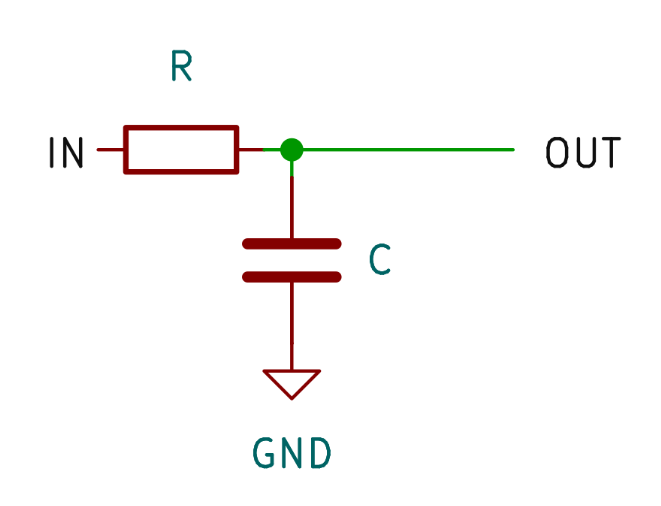
\includegraphics[width=0.49\linewidth]{low-pass-RC.png}%
    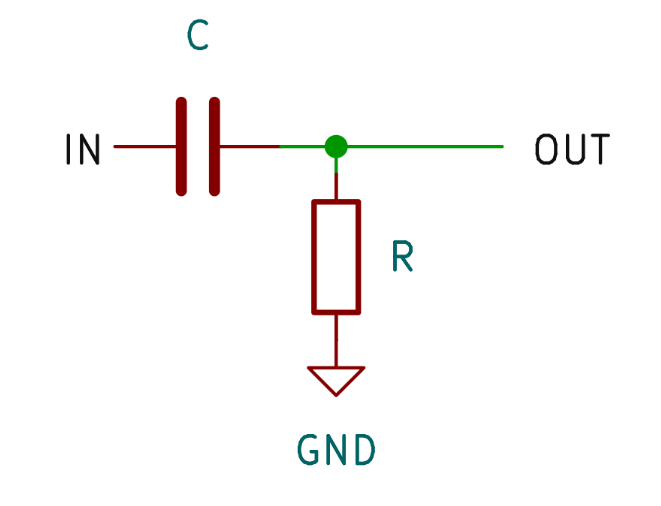
\includegraphics[width=0.49\linewidth]{high-pass-RC.png}%
    \label{fig:RC-lowpass}
    \caption{Low-pass (left) and high-pass (right) RC filter.}
\end{figure}

Using the impedance of a capacitor $Z_C = (i\omega C)^{-1}$ for voltage oscillating at angular frequency $\omega$, we get for the low-pass filter
\begin{equation}
    \frac{V_\mathrm{out}}{V_\mathrm{in}} = \frac{1}{1 + i\omega RC},
\end{equation}
and for the high pass
\begin{equation}
    \frac{V_\mathrm{out}}{V_\mathrm{in}} = \frac{i\omega RC}{1 + i\omega RC}.
\end{equation}
The above expressions are called transfer functions of the filter. Quantity $RC = \tau$ is called the time constant. The corner frequency $f_c = 1/(2\pi\tau)$ is the frequency when the filter starts acting. We can plot the response of the filters with the following code
\lstinputlisting[firstline=4,lastline=12,caption={RC filter response}]{../example_code/RC_filters_response.py}
\begin{center}
    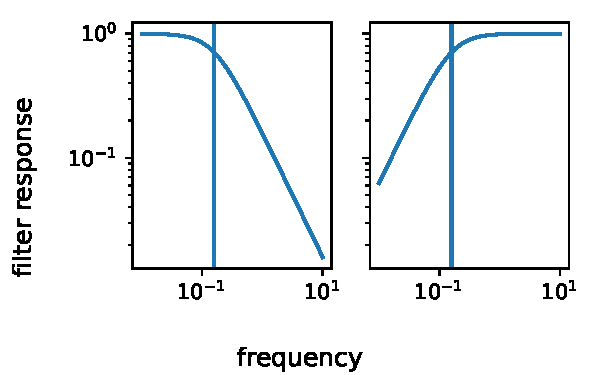
\includegraphics{RC_filters.pdf}
\end{center}
The figure shows the absolute value of the transfer function for the low-pass and high-pass RC filters, respectively. The vertical line is the corner frequency.

Notice that the transfer functions are functions of frequency and the circuits they represent are linear, i.e. they act on each frequency independently. Therefore, if $s(t)$ is our signal and $\hat s(f)$ is its Fourier transform, the Fourier transform of the signal filtered with a transfer function $H(f)$ is simply
\begin{equation}
    \hat s'(f) = H(f)\hat s(f),
\end{equation}
i.e., filters in frequency domain simply multiply the spectrum. In time domain $s'(t) = \mathcal{F}^{-1}[H\hat s]$; Fourier transform of a multiplication is a convolution, i.e.
\begin{equation}
    s'(t) = (h*s)(t) \equiv \int_{-\infty}^t s(t')h(t - t')\dd t,
\end{equation}
where $h$ is the inverse Fourier transform of $H$ and is called the convolution kernel. Note that FFT is often the fastest way to calculate a convolution, although we do not have to implement it ourself since there is \ls{scipy.signal.convolve(a, b)}, which calculates the convolution of signals \ls{a} and \ls{b}.

For the low-pass RC filter it can be proven that
\begin{equation}
    h(t) = \left\{\begin{matrix}
        e^{-t/\tau} & \mathrm{for}\; t > 0 \\
        0 & \mathrm{for}\; t < 0
    \end{matrix}\right.
\end{equation}
which can also be easily implemented for streaming data, for which it is often called \emph{exponential smoothing}.

Apart from low-pass and high-pass filters there are also band-pass and band-stop filters. Band-pass only lets through a certain frequency band (i.e., an interval) and band-stop lets through everything except for a certain frequency band. You can imagine band-pass as a high-pass followed by a low-pass in series and band-stop as a low-pass and high-pass in parallel with corner frequencies given by the pass or stop band. 

The simple RC filters above are so-called first order. The order of the filter indicates how fast it cuts the signal outside of the \emph{pass band} (i.e., the interval of frequencies which the filter lets through). This is often measured in decibels per octave (dB/oct) which indicates by how many decibel is the signal attenuated if its frequency doubles, for a low-pass filter, or halves for high-pass filter, sufficiently far from the corner frequency. Both of the RC filter are 6 dB/oct, since every doubling of frequency remove 6 dB of transmitted power.

Faster filters can be constructed both electronically and digitally, but as you saw in the examples with the step function, sharp cutoff in the spectrum leads to oscillations, which are typically undesirable. The filters that are maximally flat in the pass-band are the Butterowrth filters, named after Stephen Butterowrth, which have amplitude gain
\begin{equation*}
    G_n(\omega) = \frac{1}{\sqrt{1 + \frac{\omega^{2n}}{\omega_c^{2n}}}},
\end{equation*}
where $\omega_c$ is the corner (angular) frequency. We can construct these filters using \ls{scipy.signal.iirfilter} and apply it to our signal using \ls{scipy.signal.sosfilter}
\lstinputlisting[firstline=7, lastline=25, caption={Using IIR filter.}]{../example_code/sig_iirfilter.py}:
\begin{center}
    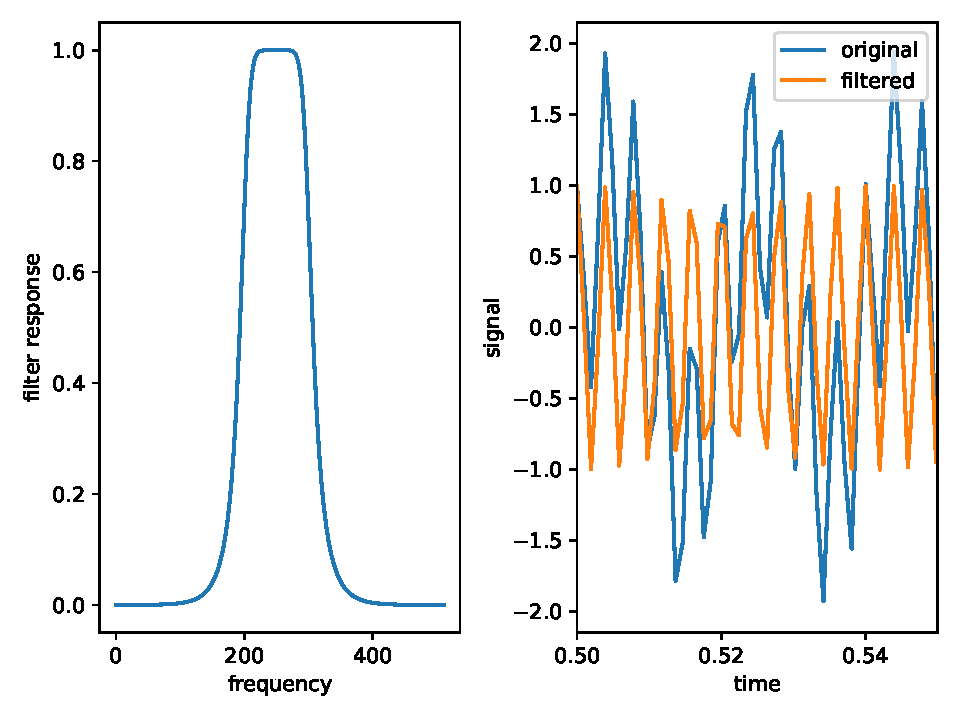
\includegraphics[width=0.5\linewidth]{butter.pdf}
\end{center}

\begin{exercise}
    \label{ex:filter}
    Write a function, which will filter the input signal using
    \begin{enumerate}
        \item low-pass RC filter with adjustable cutoff frequency
        \item high-pass RC filter similarly to 1.
        \item Butterworth band-pass filter constructed using \ls{scipy.signal.iirfilter()} and applied using \ls{scipy.signal.lfilter()}
    \end{enumerate}

    For 1. and 2. plot the the filter transfer function. Test the filtering on the attached \ls{noisy_data.npy} and plot the signal in both the time and frequency domain before and after filtering. For the low-pass filter, filter out everything above 100 Hz. For high-pass, everything below 1000 Hz and for band-pass leave only the range (4310, 4330) Hz.
\end{exercise}

% \subsection{Homodyne and heterodyne detection, signal envelope}
% TODO: mixing, homodyne and heterodyne detection, lock-in amplification

\begin{exercise}
    \label{ex:envelope-direct}
    Demodulate the cleaned-up signal from Exc.~\ref{ex:filter} (using Butterworth band pass filter) on the carrier frequency 4321 Hz (multiply by $e^{i\omega t}$ and low-pass filter) and plot the envelope modulating the carrier wave.
\end{exercise}

\begin{exercise}
    \label{ex:envelope-hilbert}
    Calculate the signal envelope from Exc.~\ref{ex:envelope-direct} using the Hilbert transform.
\end{exercise}

\subsection{Interpolation and smoothing.}

TODO: \ls{scipy.ndimage.gaussian_filter()}, \ls{scipy.signal.savgol_filter()}, \ls{scipy.interpolate.interp1d()}, \ls{scipy.interpolate.UnivariateSpline()}